
\chapter{Theoretical Background}\label{theoretical-background}

A variety of sensors enable robots to sense their environment. Most robots monitor proprioceptive (i.e. self-sensing) information like odometry from intertial measurement units (IMU) and wheel encoders. This section focuses on how a robot can avoid or detect collisions with exteroceptive (i.e. environment-sensing) sensors.

\section{Traditional Obstacle Sensors}\label{traditional-obstacle-sensors}

The fallback option of obstacle sensing is almost always a bumper
sensor. If the robot runs into an obstacle in its path, a bumper switch
will be pressed and the robot's navigation system knows that it can not
traverse further in this particular direction. The concept can be
extended to measure sudden acceleration that indicates a collision or
even monitor motor current to find that the robot is stuck against an
obstacle, but the idea is the same: With this kind of sensor, the robot
can only detect that it already had a collision. The detection can be
shifted to a slightly earlier point in time with whisker-like
antennae or capacitive sensors \cite{Muhlbacher-Karrer2015}. A special
case is negative obstacle (e.g.~cliff) detection. Here, infrared
(IR) range sensors are usually employed on the underside of the robot.

Intelligent navigation and path planning however can only be achieved
with ranging sensors. Classic range sensors are IR-, ultrasound (US)-, or
laser-based. They measure the distance to the closest target in one
direction. Because obstacles can appear in any direction, these sensors
need to be scanned. Scanning means that the bearing of active sensing
direction is changed over time to achieve range scans that are
multiplexed over a field of view (FOV). Usually this is done
mechanically, with a sensor turret spinning on a servo motor. The best
known example of this is the classic lidar sensor, which spins a laser
range finder around.

Vision sensors are scannerless and include regular cameras as monocular
vision sensors and stereo-camera setups to record depth
information. Structured light sensors such as the first-generation
Microsoft Kinect sensor record depth disparity from triangulation, via
correlation between a known and perceived projected light pattern.
Time-of-flight (TOF) cameras like the second-generation Microsoft Kinect
illuminate the scene with amplitude-modulated near-IR light and
calculate depth from the phase shift between the transmitted and
received signal \cite{Sarbolandi2015}.

There is also a scannerless version of lidar. Full-field lidar, also
known as flash lidar \cite{Payne2008}, uses TOF measurements of
omnidirectional light pulses to capture a 2D scene.

To map out the environment and localize itself, the robot will usually
employ a version of a slam algorithm \cite{Cadena2016} --- After years of being a research field, slam is now finally showing up in products.

\Cref{fig:lidar_rgbd} shows a situation where a robot's laser scanner only detects a single point (green) on the pillar of an office chair. The resulting gridmap will feature a single occupied cell at this location, but the horizontal chair legs are completely undetected. In practice, the robot often bumps into the ``invisible'' chair legs and sometimes gets stuck while navigating in this environment. These horizontal chair legs can be detected with a depth camera, which is the source of the chair's 3D image and the 3D occupancy grid in \cref{fig:lidar_rgbd}. The vision/depth sensor is however also not perfect: A decent amount of processing power is necessary to run a visual slam; but the bigger problem is that some obstacles are still not visible. In \cref{fig:rgbd_glasswall}, chairs behind the window and a part of the window frame are recognized, but the glass wall is literally completely transparent.

\begin{figure}
    \begin{subfigure}[t]{.485\textwidth}
        \centering
        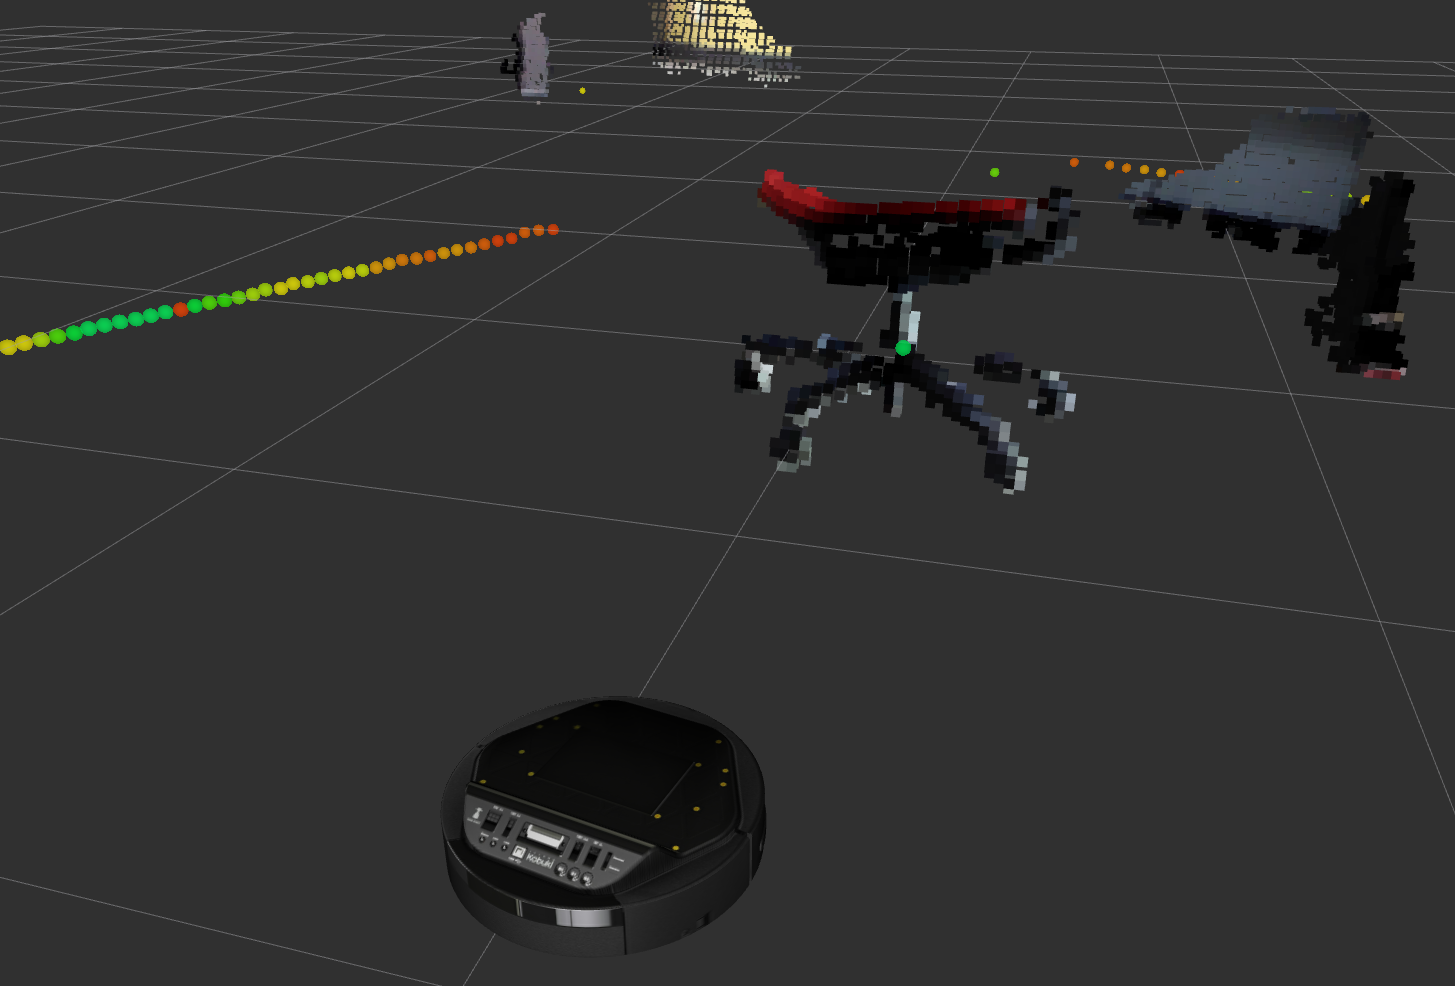
\includegraphics[max width=\textwidth]{gfx/screenshots/chair_laser_vs_rgbd}
        \caption{Laser fails to detect horizontal chair legs.}
        \label{fig:lidar_rgbd}
    \end{subfigure}%
    \hfill%
    \begin{subfigure}[t]{.485\textwidth}
        \centering
        \def\svgwidth{\linewidth}
        \input{gfx/screenshots/rgbd_glasswall.pdf_tex}
        \caption{RGBD camera can not detect glass surface.}
        \label{fig:rgbd_glasswall}
    \end{subfigure}%
    \caption{Screenshots showing traditional sensor shortcomings.}
\end{figure}

\section{Radar Sensing}\label{radar}

Radar sensing is based on the transmission and reflection of
electromagnetic signals. A transmitting antenna radiates EM energy, some
of which is scattered off reflective objects, called targets, and
intercepted by a receiving antenna. This signal is amplified and checked
for time delay, frequency shift, phase shift and amplitude attenuation
with respect to the transmitted signal. This allows to capture certain
target properties like range, radial velocity, size, shape and, among
others, even surface smoothness and orientation \cite{Skolnik2008}.

\begin{minipage}{\textwidth} % keep this together
The return signal's echo power is described for the interference-free
case in vacuum by the radar equation,
\begin{equation} \label{eq:radar}
    P_r =  \frac{P_t G_t}{4\pi R^2} \cdot \frac{\sigma}{4\pi R^2} \cdot A_r
\end{equation}
where
\begin{tabbing}
\hspace{1cm} \= \kill
$P_r$ \> received target echo power \\
$P_t$ \> transmission power \\
$G_t$ \> transmit antenna gain \\
$R$ \> range of target (distance) \\
$\sigma$ \> radar cross section (RCS) of target \\
$A_r$ \> effective area of receiving antenna.
\end{tabbing}
\end{minipage}

Of the three factors in the equation, the first
factor represents the power density at the radar-illuminated target's
distance. The second factor represents how much of the radar energy is
scattered back by the target. The third factor denotes how much
of the echo power is collected by the receiving antenna.
\cite{Skolnik2008} Conventional radar only becomes useful with directive
antennas. The antenna gain \(G_t\) is defined as the ratio of increased
power in a particular direction compared with that from an isotropic
antenna \cite{Adams2012}. Antenna theory shows \cite{Balanis2015} the
relation of receive antenna gain \(G_r\) with radiation wavelength
\(\lambda\):
\begin{equation} \label{eq:recvgain}
    G_r = \frac{4\pi A_r}{\lambda^2}    
\end{equation}
With constant antenna loss factor \(L>1\), substituting \cref{eq:recvgain} into \cref{eq:radar}
yields the classical radar equation
\begin{equation} \label{eq:radarclassical}
    P_r =
    \frac{P_t G_t G_r \lambda^2 \sigma}{(4\pi)^3R^4L}
    \propto \frac{\sigma}{R^4}
\end{equation}
In practice, the actual received power is lower than predicted by
this equation due to many factors including interference and
atmospheric conditions. \(\sigma\) is also not constant but varies with
viewing angle and material properties of the target. \cite{Adams2012}

\subsection{Doppler effect}\label{doppler-effect}

Many radar systems measure radial velocity with the Doppler frequency
shift. Austrian physicist Christian Doppler described the kinematic
effect in 1842. It describes the change of wavelength caused by the
motion. A common example is the change of pitch that can be heard when a
race car or ambulance passes the observer. The Doppler frequency shift
\(f_D\) is
\begin{equation} \label{eq:doppler}
    f_D = 2 \frac{v_r}{\lambda} = 2 \frac{v \cos ( \theta )}{\lambda}
\end{equation}
where \(v_r\) is the radial velocity component of the target, which
travels at a speed \(v\) at angle \(\theta\) between the target's
direction and the radar beam with wavelength \(\lambda\)
\cite{Skolnik2008}. The factor \(2\) is caused by the Doppler shift
being applied twice; once for the incident wave, and once for the
reflected wave. In effect this means that a radar sending out an EM wave
with a frequency of exactly \SI{60}{GHz} towards a target moving at a
relative speed of \(v_r = \SI[per-mode=symbol]{1}{cm\per s}\) towards the radar will receive
back an echo with a frequency of \SI{60000000004}{Hz} because of the
frequency shift of \(f_D = \SI{4}{Hz}\).

\subsection{Types of Radar}\label{types-of-radar}

\subsubsection{Continuous Wave radar}\label{continuous-wave-cw-radar}

Continuous wave (CW) radar is the earliest radar system. It uses a continuous transmission
at a fixed frequency. Thanks to antenna directionality it can find a target's azimuth in radio direction finding. A target's velocity
information can be extracted from the frequency shift due to the Doppler
effect.

\subsubsection{Pulse radar}\label{pulse-radar}

Pulse radars send series of short bursts. The time delay \(\tau\)
between transmission and reception of a pulse is called time of flight
(TOF). Together with speed fo light $c$ it yields a target's range \(R\):
\begin{equation} \label{eq:tof}
	 R = \frac{c\tau}{2} 
\end{equation}
The range resolution \(\Delta R\) is given by

\begin{equation} \label{eq:tof_res}
	\Delta R = \frac{c\tau_m}{2}
\end{equation}
with \(\tau_m\) the pulse high time of the burst modulation (see \cref{fig:radar_pulse}). To
achieve high range resolution pulses must be very short, which requires
very high peak transmission power to still produce a detectable echo
signal. Pulse compression radars send a longer pulse with an internal
modulation, which combines the higher transmission energy of longer
pulses with the resolution of short pulses. Velocity is again known from
frequency shift.

\begin{figure}[htp]
    \centering
    \def\svgwidth{10cm}
    \input{gfx/diagrams/radar_pulsed.pdf_tex}
    \caption{Pulse radars measure the time between transmission and reception of a short EM burst. Adapted from \cite{Adams2012} p.~52.} \label{fig:radar_pulse}
\end{figure}


\subsection{Frequency-modulated continuous wave (FMCW) radar}\label{frequency-modulated-continuous-wave-fmcw-radar}

FMCW radars use a frequency modulation to measure range and speed at the
same time. The transmitted modulation is compared to the modulation in
the received signal to detect signal delay and frequency shift.
Applications in robotics use this kind of radar the most, for reasons of
lower transmission power and high-range resolution \cite{Adams2012}.

An FMCW radar's modulation is called a frequency sweep or chirp and is
usually triangular with a linearily increasing and decreasing frequency.
Most sensor use a voltage controlled oscillator (VCO) to generate the
modulation waveform. VCOs do not have a linear transfer function, so in
order to obtain a linear sweep, the input to the VCO must be
pre-distorted with the inverse of the VCO's nonlinear transfer function.
Instead of a VCO, direct digital synthesizers together with phase-locked
loops (PLL) can be used. They generate better (more linear) sweeps at
the price of increased design complexity and cost \cite{Ernst2016}.

\begin{figure}[htp]
    \centering
    \def\svgwidth{\linewidth}
    \input{gfx/diagrams/fmcw_blocks.pdf_tex}
    \caption{\label{fig:fmcw_blocks}Simplified FMCW architecture. Adapted from \cite{VanZeijl2014}.}
\end{figure}

After the VCO's signal is amplified and transmitted, it reflects at
visible targets and is received as echo in the same frequency band.

\begin{figure}[htp]
    \centering
    \def\svgwidth{10cm}
    \input{gfx/diagrams/fmcw_triangular.pdf_tex}
    \caption{\label{fig:fmcw_triangular}FMCW radars detect targets in the beat frequency, which is a frequency mix of the transmitted and received modulation. Adapted from \cite{Adams2012} p.~57.}
\end{figure}

\Cref{fig:fmcw_triangular}'s top subplot shows the transmitted frequency sweep
from \(f_0\) to \(f_0 + \Delta f\) over a sweep length of \(T_d\) of a
triangular modulation. The middle plot also shows the received signal as
caused by a single stationary ideal reflector. Time of flight causes a
delay \(\tau\) in the received signal. To understand where the beat
signal comes from, we focus on the rising part of the triangle
modulation, the upsweep. Using the superheterodyne principle the
received signal \(v_{Rx}\) and a portion of the transmitted signal
\(v_{Tx}\) (called the local oscillator (LO)), are frequency mixed in an
analog multiplier to get the intermediate frequency (IF) \(v_{Mixer}\).
The IF contains a target's beat frequency, which is proportional to the
target's range. With the transmitted signal \(v_{Tx}\) and the received
signal \(v_{Rx}\) as a function of time \(t\), 
\begin{align}
    v_{Tx}(t) &= A_{Tx} \cos\bigl(\omega_{Tx}(t)~t\bigr) \label{eq:fmcw1} \\
    v_{Rx}(t) &= A_{Rx} \cos\bigl(\omega_{Tx}(t-\tau)~t\bigr) \label{eq:fmcw2}
\intertext{where}
    \omega_{Tx}(t) &= \underbrace{\omega_c}_\text{Carrier frequency} + \underbrace{\pi \frac{\Delta f}{T_d} t}_\text{Upsweep modulation} \nonumber
\end{align}

is the (angular) frequency of the transmitted signal. The signal \(v_{Mixer}\) behind the frequency mixer can be calculated as the mix (i.e. multiplication) of $v_{Tx}(t)$ and $v_{Rx}(t)$ from \cref{eq:fmcw1,eq:fmcw2}:
\begin{align}
\begin{split}
    v_{Mixer}(t)    &= v_{Tx}(t) ~ v_{Rx}(t) \label{eq:fmcw3}\\
                    &= A_{Tx}A_{Rx}~\cos(t\omega_{Tx}(t))t~\cos(\omega_{Tx}(t-\tau)t)
\end{split}
\end{align}

With the trigonometric identity
\begin{equation*}
	 \cos A \cdot \cos B = \frac{1}{2} \Bigl( \cos(A+B)~+~\cos(A-B) \Bigr)
\end{equation*}

\cref{eq:fmcw3}'s \(v_{Mixer}\) can be rewritten as 
\begin{equation*}
	v_{Mixer}(t-\tau) = \frac{A_{Tx} A_{Rx}}{2}(B_1 + B_2)
\end{equation*}
where
\begin{align}
	B_1 &= \cos\left[ \vphantom{\frac{\Delta f}{T_d}} 2\omega_{Tx}(t-\tau) t - \omega_{Tx}(\tau)\tau \right] \nonumber \\
        &= \cos\left[ 2\left(\omega_c + \pi\frac{\Delta f}{T_d}(t-\tau)\right)t - \left(\omega_c - \pi\frac{\Delta f}{T_d}\tau\right)\tau \right]\\
    B_2 &= \cos\left[ 2\left(\pi\frac{\Delta f}{T_d}t\right)\tau - \omega_{Tx}(\tau)\tau \right]  \nonumber \\
        &= \cos\left[ 2\pi\left(\frac{\Delta f}{T_d}\tau\right)t - \left(\omega_c + \pi\frac{\Delta f}{T_d}\tau\right)\tau \right] \label{eq:fmcw4}
\end{align}

Note that \(B_1\) consists of high angular frequencies around the
carrier frequency, from \(f_0 = \frac{\omega_c}{2\pi}\) to
\(f_0 + \Delta f\). \(B_2\) is a lower frequency (theoretically up to
\(2\pi\Delta f\) at \(\tau = T_d\), but much lower in practice, as echos
from targets this far away have very low intensity \(A_{Rx}\) and can't
be detected) signal containing the beat frequency. The output of the
low-pass filter intrinsic in the mixer stage will thus only consist of
the beat frequency (plus noise of similar frequencies) from \cref{eq:fmcw4}:
\begin{equation} \label{eq:vbeat}
    v_{beat}(t,\tau) = \frac{A{Tx}A_{Rx}}{2} \cos \left[ 2\pi\left(\frac{\Delta f}{T_d}\tau\right)t - \left(\omega_c + \pi\frac{\Delta f}{T_d}\tau \right) \tau \right]
\end{equation}

The term \(\frac{\Delta f}{T_d}\tau\) in \cref{eq:vbeat}'s \(v_{beat}(t,\tau)\) is
known as the beat frequency \(f_b\). For stationary targets, the
range-specific frequency \(f_R = f_b\). Knowing that the delay time
\(\tau\) depends on the speed of light \(c\) and the range \(R\), the
relationship between a target's \(f_R\) and range \(R\) can be given as

\begin{equation}\label{eq:range}
	f_R = \frac{2R}{c} \frac{\Delta f}{T_d} \iff R=\frac{c T_d}{2\Delta f}f_R
\end{equation}

This also gives the range resolution \(dR\),

\begin{equation} \label{eq:rangeres}
	dR = \frac{c}{2 \Delta f}
\end{equation}

A moving target however will introduce a Doppler shift \(f_D\) in the
received signal \(v_{Rx}\), which will shift the target's beat frequency
\(f_b\) away from its range-specific frequency \(f_R\). The direction of
the frequency shift depends on the modulation: An up-sweep will have a
corresponding $f_{b,up}$, while the down-sweep will have $f_{b,down}$
\begin{align}
	f_{b,up}    &= f_R - f_D \label{eq:vbeatup} \\
	f_{b,down}  &= f_R + f_D \label{eq:vbeatdn}
\end{align}

\begin{figure}[htbp]
    \centering
    \def\svgwidth{10cm}
    \input{gfx/diagrams/fmcw_doppler.pdf_tex}
    \caption{\label{fig:fmcw_doppler}Target motion introduces a Doppler shift in the received signal, which changes the beat frequency during up- and down-sweeps. Adapted from \cite{Adams2012} p.~57.}
\end{figure}

The range-specific frequency and Doppler frequency can be extracted from the two beat frequencies of \cref{eq:vbeatup,eq:vbeatdn} by averaging them: 
\begin{align}
	f_R &= \frac{f_{b,down} + f_{b,up}}{2} \\
    f_D &= \frac{f_{b,down} - f_{b,up}}{2}
\end{align}
The benefit of the triangular sweep becomes clear here: with a sawtooth
waveform, only \(f_b,up\) can be determined. A stationary target and a
moving target a range and Doppler speed corresponding to the same
resulting frequencies would not be distinguishable.

Of course, more than one target can be visible at a time. If multiple
echos are received, as in \cref{fig:fmcw_multitarget}, the intermediate frequency will
contain multiple frequencies. The beat signal will have more than one
dominant frequency in its spectrum, with each one corresponding to a
different target.

\begin{figure}[htbp]
    \centering
    \def\svgwidth{10cm}
    \input{gfx/diagrams/fmcw_multitarget.pdf_tex}
    \caption{By reflecting a portion of the transmission signal back to the radar, each target (green, yellow and blue lines) contributes a frequency corresponding to its range in the beat spectrum / range response.}
    \label{fig:fmcw_multitarget}
\end{figure}

Finally, with the help of \cref{eq:range}, this frequency spectrum can be interpreted as range profile, with every target's dominant frequency corresponding to the target's range.

\Cref{fig:fig_raw_beat} shows a real-world example of how the beat signal \(f_b\)
(\cref{fig:rawbeat_t}) and its frequency spectrum (\cref{fig:rawbeat_f}) look like. At
\(t=T_d=\SI{32}{ms}\), a jump in the beat frequency is caused by the modulation
change from upsweep to downsweep. In the frequency spectrum, three
stationary targets are visible at ca. \SI{3}{kHz}, \SI{6}{kHz}, and \SI{9}{kHz}.
In this example, \(T_d=\SI{32}{ms}\) and \(\Delta f=\SI{7}{GHz}\), so the targets were
at ranges of \SI{0.5}{m}, \SI{1}{m}, and \SI{1.5}{m}. The Fourier transform
in \cref{fig:rawbeat_f} shows the frequency spectrum's magnitude \(\|S\|\).

\begin{figure}[htbp]
    \begin{subfigure}[t]{0.475\textwidth}
        \centering
        \def\svgwidth{\linewidth} \small
        \input{gfx/fig_svg/raw_beat_1.pdf_tex}
        \caption{\label{fig:rawbeat_t}Time-domain beat signal}
    \end{subfigure}%
    \hfill%
    \begin{subfigure}[t]{0.475\textwidth}
        \centering
        \def\svgwidth{\linewidth} \small
        \input{gfx/fig_svg/raw_beat_2.pdf_tex}
        \caption{\label{fig:rawbeat_f}Beat signal frequency spectrum}
    \end{subfigure}
    \caption{\label{fig:fig_raw_beat}Beat signal and spectrum / range profile in a real-world measurement.}
\end{figure}

\subsection{Direction of Arrival}\label{direction-of-arrival}

A radar sensor with two or more receiving antennas which are separated
by not more than half a wavelength can measure the Direction of arrival
(DOA) of one or multiple targets. Because the echo from a target has to
travel a slightly longer distance to antennas further away, a phase
difference between the different antenna signals is measurable.

The basis for this is that not only the magnitude $\|S\|$ of a signal is received, but that also the in-phase component $S_I$ and quadrature component $S_Q$ of the analytic signal are measured in separate channels in order to retain phase information. This is the reason for separate \textit{RX 1 I} and \textit{RX 1 Q} signals in \cref{fig:rawbeat_t}. \Cref{fig:iq} shows how the two components make up the complex signal. The physical reason for the two parts existing is the oscillation of the radar wave's EM energy between electric and magnetic fields. The frequency $f$ of the wave determines the speed of the oscillation and the phase $\phi$ indicates at which point in this oscillations cycle the wave currently is. As the propagation speed of the wave is limited to the speed of light $c$, two spatially separated antennas receive the same signal at different oscillation phases. This difference is the phase difference $\Delta\phi$. Other than the spatial antenna separation $d$, $\Delta\phi$ only depends the wave's frequency $f$ (or wavelength $\lambda$) and the direction of arrival $\theta$ (see \cref{fig:doa}).

\begin{figure}[htbp]
    \begin{subfigure}[t]{0.5\textwidth}
        \centering
        \def\svgscale{1}
        \input{gfx/diagrams/IQ.pdf_tex}
        \caption{I/Q signal with phase $\phi$}
        \label{fig:iq}
    \end{subfigure}
    \begin{subfigure}[t]{0.5\textwidth}
        \centering
        \def\svgscale{1}
        \input{gfx/diagrams/doa.pdf_tex}
        \caption{Direction of Arrival \(\theta\) can be estimated from phase difference \(\Delta\phi\)}
        \label{fig:doa}
    \end{subfigure}
    \caption{Phase difference and I/Q signal}
    \label{fig:doiq}
\end{figure}

Viewing a complex analytic received signal $S$ at time $t$,
\begin{align} \label{eq:analytic}
    S(t) &= S_I(t) + j~S_Q(t)
\intertext{as}
    S(t) &= A_{Rx}~\exp(j\phi) \nonumber
\end{align}
explains why the phase difference $\Delta\phi$ can be calculated from the complex angle difference of the complex analytic antenna signals $S_{Rx1}$ and $S_{Rx2}$ at antennas \textit{Rx1} and \textit{Rx2}, respectively:
\begin{equation} \label{eq:phasediff}
    \Delta\phi = \angle S_{Rx1} - \angle S_{Rx2}
\end{equation}

With \cref{eq:phasediff}'s $\Delta\phi$ direction of arrival $\theta$ can be estimated \cite{VanZeijl2014} as
\begin{equation} \label{eq:doa}
	\theta = sin^{-1}\left({\frac{\lambda~\Delta\phi}{2\pi ~d}}\right)
\end{equation}

DOA estimation has been thoroughly studied and many algorithms have been designed and evaluated, including subspace-based decorrelation methods like MUSIC and ESPRIT \cite{Schmidt1986,Tang2014,Paulraj1985}, and beamforming techniques like Bartlett and Capon \cite{Krishnaveni2013,Capon1969} and others like the method of minimum phase error proposed by Cho \textit{et al.} in \cite{Cho2017}. The presented approach is a simplified two-antenna version of \cite{Cho2017}. The implementation that will be detailed in \cref{implementation} does not require a very accurate $\theta$ but relies mostly on $\sgn(\theta)$. Results in \cref{results} show however that $\theta$ is a reasonable estimation that holds well for strong signals.

\subsection{Frequencies}\label{frequencies}

Even though radar applications exist for many frequencies, only a few of
them are OK to use for radiolocation and in home robots. The
``Industrial, Scientific, Medical'' (ISM) bands allow the unlicensed
use of some frequencies for radiolocation, including center frequencies
of \SI{24.125}{GHz}, \SI{61.25}{GHz}, \SI{122.5}{GHz} and \SI{245}{GHz}.
Applications must, however, accept harmful interference \cite{FCC2017}.

The \SI{77}{GHz} band is ``restricted to vehicle-mounted field disturbance
sensors used as vehicle radar systems.'' (FCC Part 15 §15.253(c)). The European Telecommunications Standards Institute (ETSI)
defines it as ``Automatic Cruise Control `long-range radar' operating at
\SI{77}{GHz}. This enables a vehicle to maintain a cruising distance from
a vehicle in front.'' (EN 301 091). The German Bundesnetzagentur also
declares it ``Kraftfahrzeug-Kurzstreckenradar'' (Vfg 66 / 2014).

A \SI{24}{GHz} center frequency is a safe bet. There are many radar
systems available and it being an ISM band makes licensing much easier.
The drawback is the very limited maximum bandwidth of \SI{250}{MHz} in this
band.

Some newer radars use the \SI{60}{GHz} ISM band. It allows a rather wide
bandwidth of up to \SI{9}{GHz} in some regions (see \cref{fig:wigig} ).
According to \cref{eq:rangeres}, this gives a very good range resolution in
the order of a few \si{cm}. At these high frequencies, RF energy
attenuation in material increases noticeably \cite{FerrisJr.1998}. The
effect is that \SI{60}{GHz} waves are limited to short ranges of a few
\si{m} and don't usually penetrate walls.

Atmospheric attenuation also limits long-range applications. At short
ranges it should however not present a problem. This is why
these high frequencies are often used in indoor applications with transmission paths of not more than a few \si{m}.

\begin{figure}[htbp]
    \centering
    \begin{subfigure}[b]{0.475\textwidth}
        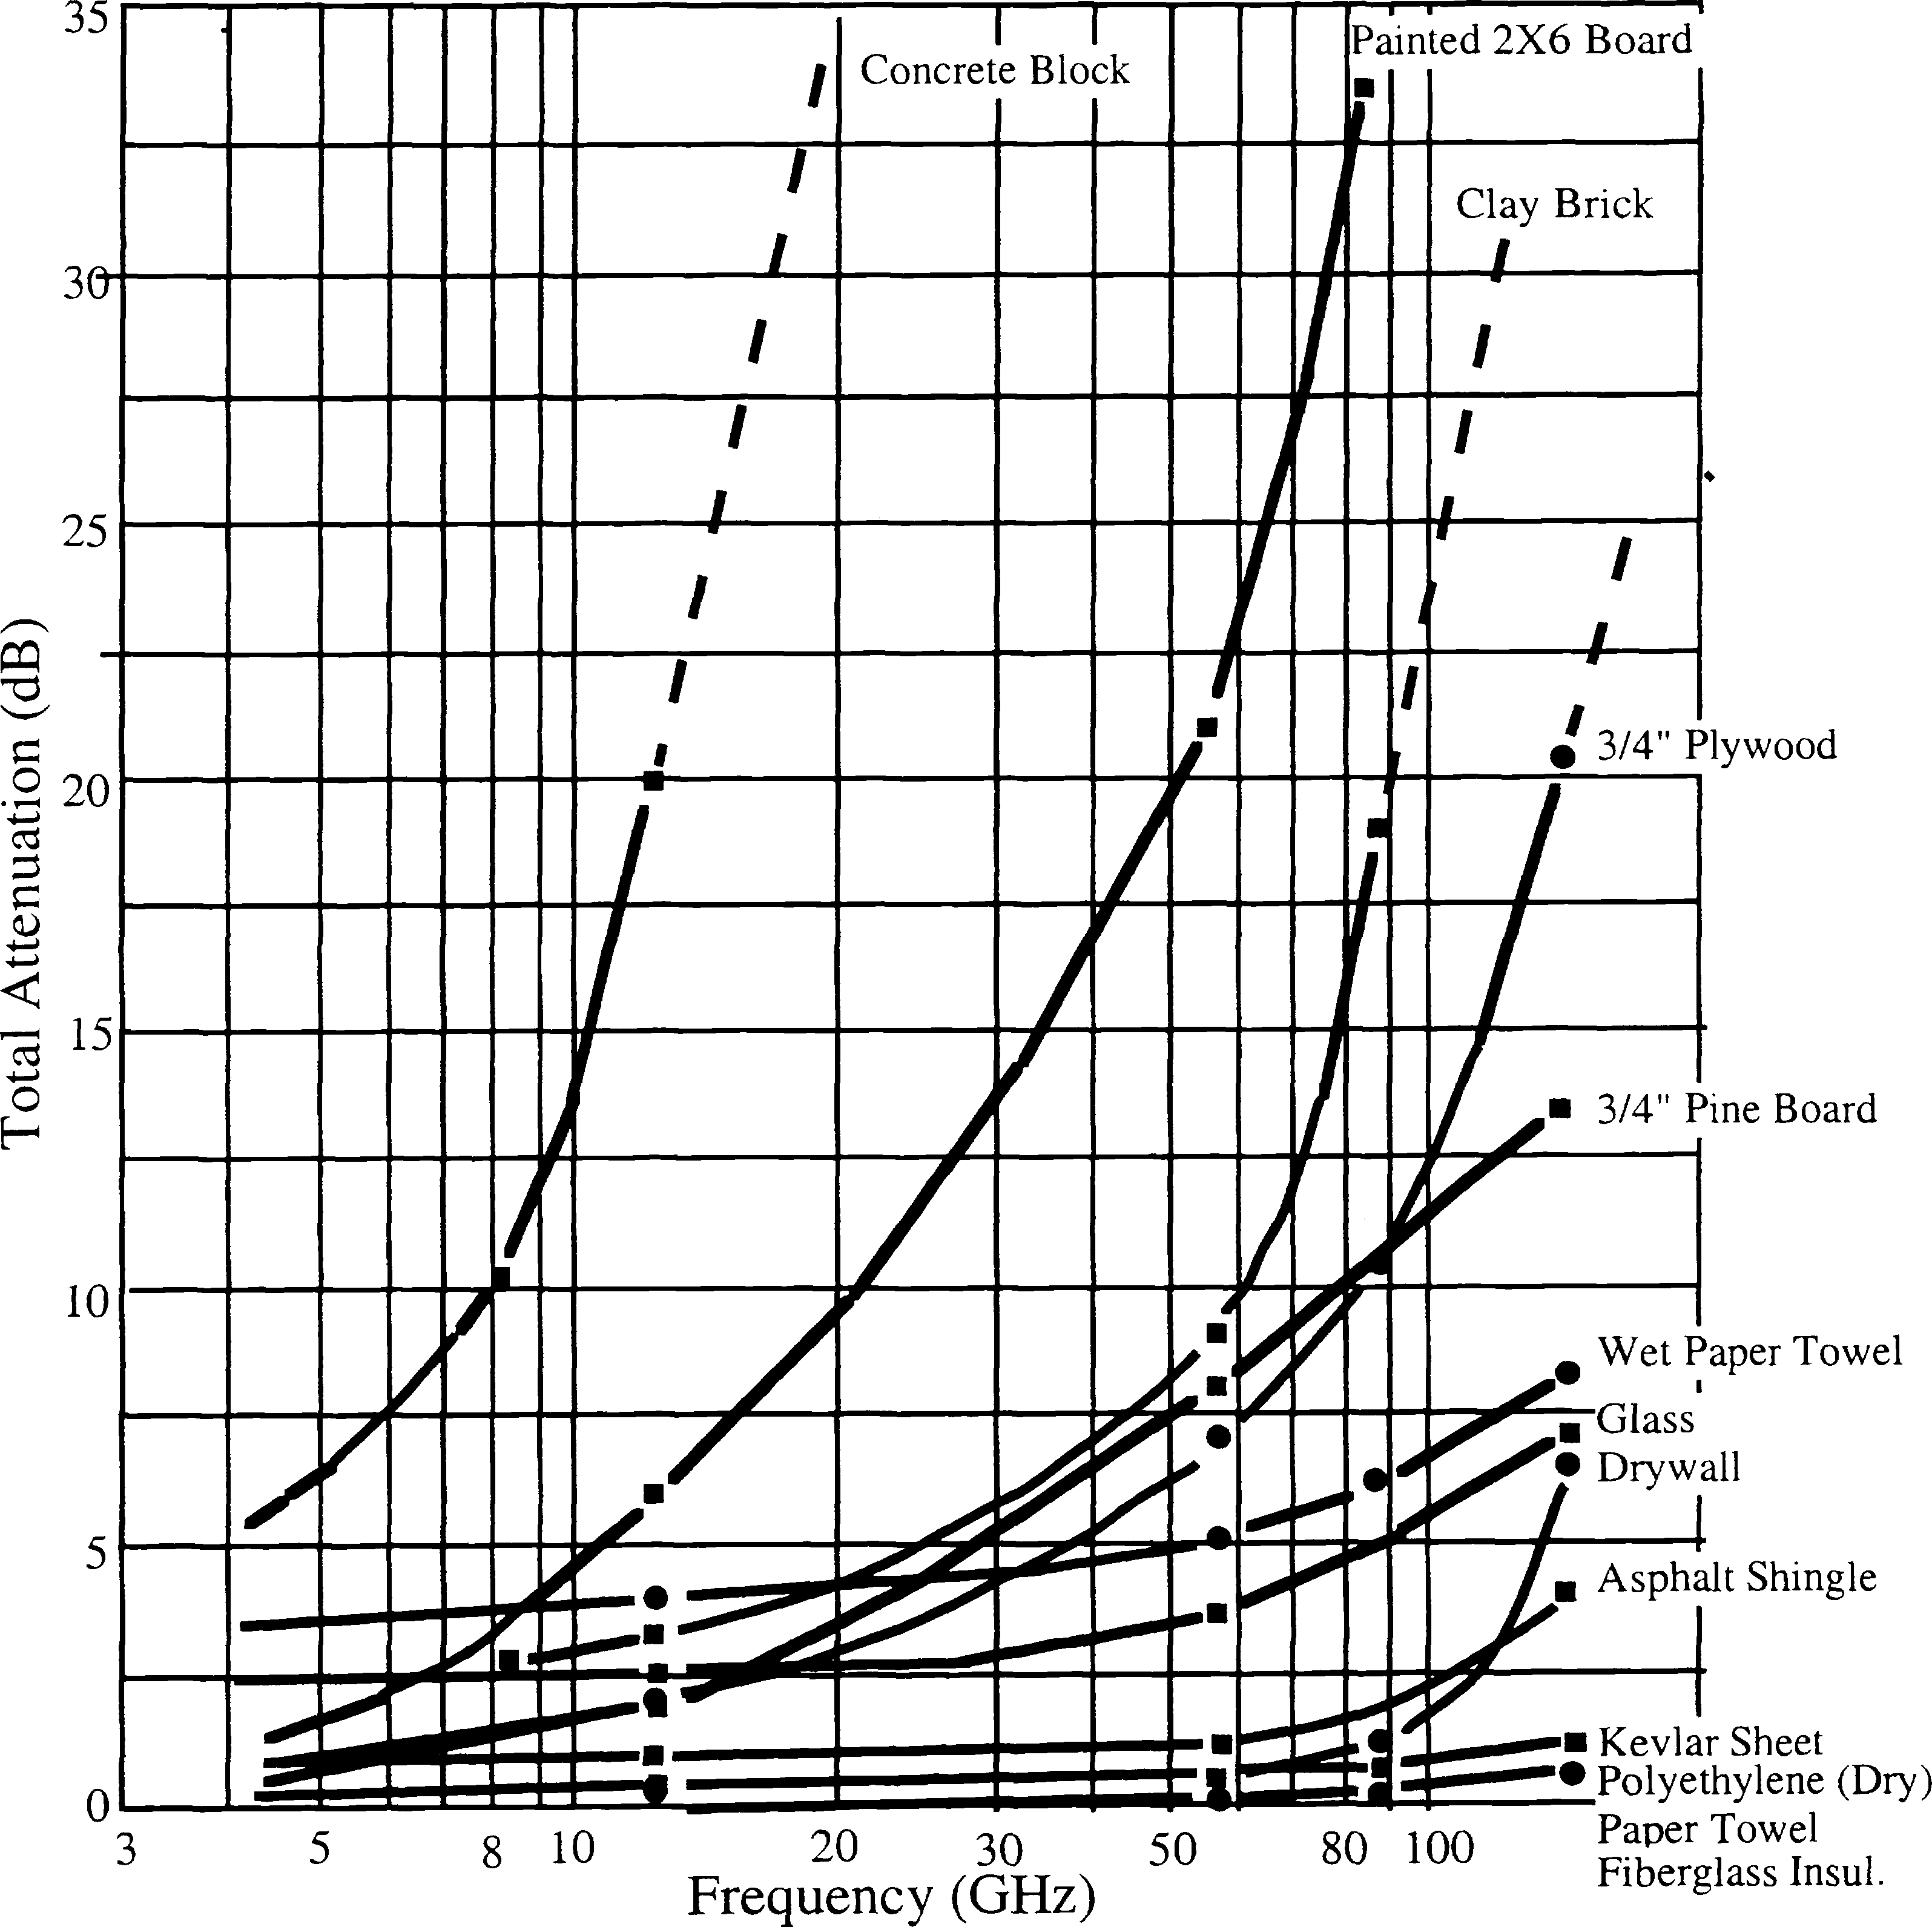
\includegraphics[width=\linewidth]{figures/rf_attenuation}
        \caption{\label{fig:attenuation}Total attenuation of RF energy when transmitted through various materials as a function of frequency. Source: \cite{FerrisJr.1998}}
    \end{subfigure}
    \hfill
    \begin{subfigure}[b]{0.475\textwidth}
        \def\svgwidth{\linewidth} \footnotesize
        \input{gfx/figures/ITU_0676-05.pdf_tex}
        \caption{\label{fig:attenuation_air}Specific RF attenuation due to atmospheric gases. Source: \cite{ITU1997}\bigskip}
    \end{subfigure}
    \caption{RF attenuation in different media.}
\end{figure}

The downside is that there are some other technologies using the same
frequency bands, most notably 802.11ad a.k.a.
WiGig \cite{AgilentTechnologies2013}. The WiGig frequency allocations in
\cref{fig:wigig} show in which regions the \SI{60}{GHz} band is available (also
for radar).

\begin{figure}[htbp]
    \centering
    \def\svgwidth{\linewidth}
    \input{gfx/diagrams/wigig.pdf_tex}
    \caption{\label{fig:wigig}WiGig Channel Plan and Frequency Allocations by Region. Source: \cite{AgilentTechnologies2013}}
\end{figure}

\section{Overview of Radar Research}\label{overview-of-radar-research}

Radar has been used and researched since the 1940s. While it was historically only used to detect aircraft and ships, it is an active research domain in many fields today.
Identification and localization of vessels is still an important application in both civil and military sectors.
There is a great amount of research going into synthetic aperture radar, in terrestrial imaging, and general and concealed imaging \cite{Cumming2004,Axelsson2002,Bury2007,Wang2008,Sarmap.ch2009,Moreira2013,Watts2016}.
Another area of research is radar antenna technology and quasi-optics, which aims to find design improvements and more adapted antennas for the manifold applications \cite{Lu2014,Tewari2015,Gorniak2008,Vinicchayakul2016,Bisognin2014,Ernst2016a,Nordin2016,Craeye2008}.
Radar is used in human presence detection and monitoring, including heartbeat detection \cite{Valmori2016,Novak2017,Zhong2016,Mabrouk2015,Ernst2016,Molchanov2011,Sakamoto2015,Molchanov2011a,Jian2014}.
A new and very promising discipline is radar-based gesture recognition, which enables innovative human machine interaction applications \cite{Lien2016,Kim2016,Molchanov2015}.
Indoor communication and localization with radar beacons is another interesting and upcoming technology \cite{Vinicchayakul2016,Albaidhani2016,Zhong2016,Zhu2016,Segura2012,Marano2010}.
The radar-related research area that is most relevant for mobile robots is radar-based slam \cite{Adams2012,Guan2017,Rapp2016,Rouveure2008,Ristic2016,Marck2013,Deissler2010,Kauffman2014,Guerra2016,Jose2004,Jose2004a,Jose2004b,Jose2005,Gerossier2009,Mullane2010,Deissler2013,Schuster2016,Adams2013,Deissler2012,Seitz2008,Deissler2010,Deissler2009}.

\section{Existing radar-based solutions for map building}\label{existing-radar-based-solutions-for-map-building}

\subsection{SAR}\label{sar}

In 1950 Doppler frequency analysis was found to improve image resolution
of side-looking radar, which led to the development of the synthetic
aperture radar (SAR) technique. SAR uses azimuth (along-track) motion to
synthesize an aperture that is longer than the physical size of the
radar antenna \cite{Wang2008}. The three major configurations are
stripmap SAR, scan SAR, and spotlight SAR. Current SAR systems can
operate in either mode by dividing their planar antenna into
sub-apertures, whose phase and amplitude are controlled by the
individual few-hundred transmit/receive modules \cite{Moreira2013}.

\begin{figure}[htbp]
    \begin{subfigure}{\linewidth}
        \centering
        \def\svgscale{1.0}
        \input{gfx/diagrams/sar_modes_strip.pdf_tex}
        \caption{Stripmap}
        \bigskip
    \end{subfigure}
    \begin{subfigure}{0.45\linewidth}
        \centering
        \def\svgscale{0.75}
        \input{gfx/diagrams/sar_modes_scan.pdf_tex}
        \caption{ScanSAR}
    \end{subfigure}
    \hfill
    \begin{subfigure}{0.45\linewidth}
        \centering
        \def\svgscale{0.75}
        \input{gfx/diagrams/sar_modes_spot.pdf_tex}
        \caption{Spotlight}
    \end{subfigure}
    \caption{\label{fig:sar_modes}Illustration of different SAR operation modes which are used to increase the swath width (ScanSAR) or improve azimuth resolution (Spotlight) compared to Stripmap mode. Adapted from \cite{Moreira2013}}
\end{figure}

Radar echo data is sampled in both fast-time and slow-time, with
fast-time meaning the range scan dimension (fast, because the EM waves
travel at very high speed, \(c\)) and slow time denoting the azimuth or
along-track dimension (slow, because movement velocity will be
\(\ll c\)). This raw data does not give any useful information and needs
to be signal-processed first. Because SAR systems typically use
pulse-compressed radars, each range line needs to be convoluted with the
complex conjugate of the transmitted chirp's spectrum to obtain the
range-compressed
data\footnote{For the FMCW system used in the later parts of this thesis this is not necessary - the FMCW beat frequency spectrum is equivalent to the range-compressed data}.
In a second step, azimuth compression takes place by convolving the
signal in slow-time with the complex conjugate of the expected
azimuth-response from a target.

\begin{figure}[htbp]
    \centering
    \def\svgwidth{\linewidth}
    \input{gfx/diagrams/sar_steps.pdf_tex}
    \caption{\label{fig_sar_steps}Summary of SAR processing steps where the range compressed data result from a convolution of the raw data with the range reference function. In a second step the azimuth compression is performed through a convolution with the azimuth reference function, which changes from near to far range. Source: \cite{Moreira2013}}
\end{figure}

An elemental scatterer at range \(R(t)\) will return an echo \(s_a(t)\)
over time \(t\): 
\begin{equation} \label{eq:scatterer}
	s_a(t) = P_r \sqrt{\sigma\vphantom{1}}
	\exp(j\varphi_s)
	\exp\Bigl(
	    j~\underbrace{\frac{-4\pi}{\lambda}R(t)}_{
	        \mathclap{ \text{ az. phase var. $\omega_D$ }}
	        }
        \Bigr)
\end{equation}
where \(P_r\) is the echo power of the received target, accounting
for dependencies like transmit power and path loss, \(\sigma\) is the
target's RCS, imaginary unit \si{j}, \(\varphi_s\) the scattering phase,
and \(\frac{4\pi}{\lambda}R(t)\) the azimuth phase variation due to
changing distance \cite{Cumming2004}. The target's range \(R(t)\) is
described by the range at closest approach \(R_0\) and the radar's
(constant) movement speed \(v_R\): 
\begin{equation} \label{eq:azphvar}
	R(t) = \sqrt{R_0^2+\left(v_Rt\right)^2} \approx R_0 + \frac{(v_Rt)^2}{2R_0} ~\text{for}~ \frac{v_Rt}{R_0} \ll 1
\end{equation}
Substituting \cref{eq:azphvar} into the azimuth phase in \cref{eq:scatterer} and derivating
with respect to time yields the azimuth frequency \(f_D\) 
\begin{equation}
	f_D = \underbrace{\frac{1}{2\pi}}_{\omega_D = 2\pi f_D} \frac{\partial}{\partial t} \frac{-4\pi}{\lambda}  \underbrace{\left( R_0 + \frac{(v_Rt)^2}{2R_0}  \right)}_{R(t)} = -\frac{2v_R^2}{\lambda R_0}t
\end{equation}
The azimuth frequency varies linearly with time \(t\) and is
inversely proportional to the closest approach (slant range) \(R_0\),
hence the azimuth reference function depends on geometry and is adapted
to range. Because of the frequency-shifting effect it is analogous to
and also called the Doppler frequency.

The most challenging aspect of SAR is the correction of range cell
migration induced defocusing. Range cell migration is visible in figure
\cref{fig_sar_steps}'s curvature of range compressed data. It occurs when a point
target's echo energy is distributed over several range cells, causing
azimuth defocusing. This effect is range-variant, as the curvature
depends on \(R_0\). Hence a non-stationary two-dimensional reference
function is necessary. There are several approaches in tackling this,
including the omega-k / wavenumber processor, range-Doppler, and chirp
scaling algorithms \cite{Moreira2013}.

As far as moved radar sensors go, SAR is a great technique for imaging a scene while it is passed on the side. If obstacle detection is to be performed, it is however necessary to know what lies ahead. Today, robots that use a radar sensor for this task therefore use a scanning radar.

\subsection{Scanning radar}\label{scanning-radar}

A radar system that changes the direction of its beam in a scanning pattern is called a scanning radar. This allows covering a larger overall search space by sampling a set of smaller regions, usually with a tighter beam shape for higher spatial accuracy. The scanning process can be implemented by mechanically rotating the radar's antenna, electronically through phased arrays (see \cref{fig:phased}), or even both in active electronically scanned arrays (AESA), which are used in fighter jets (see \cref{fig:aesa}). Some research robots use the K2PI radar sensor \cite{Rouveure2008}, which rotates a pencil-shape beam over \ang{360} (see \cref{fig:k2pi}).

\begin{figure}[htbp]
    \centering
    \begin{subfigure}[t]{0.3\textwidth}
        \def\svgwidth{\linewidth} \tiny
        \input{gfx/diagrams/phased.pdf_tex}
        \caption{The waves of a phased array's individual antennas superpose as plane wave and travel in a specific direction. Source: \url{https://wikimedia.org/wiki/File:Phased_array_antenna_system.svg}}
        \label{fig:phased}
    \end{subfigure}
    \hfill
    \begin{subfigure}[t]{0.3\textwidth}
        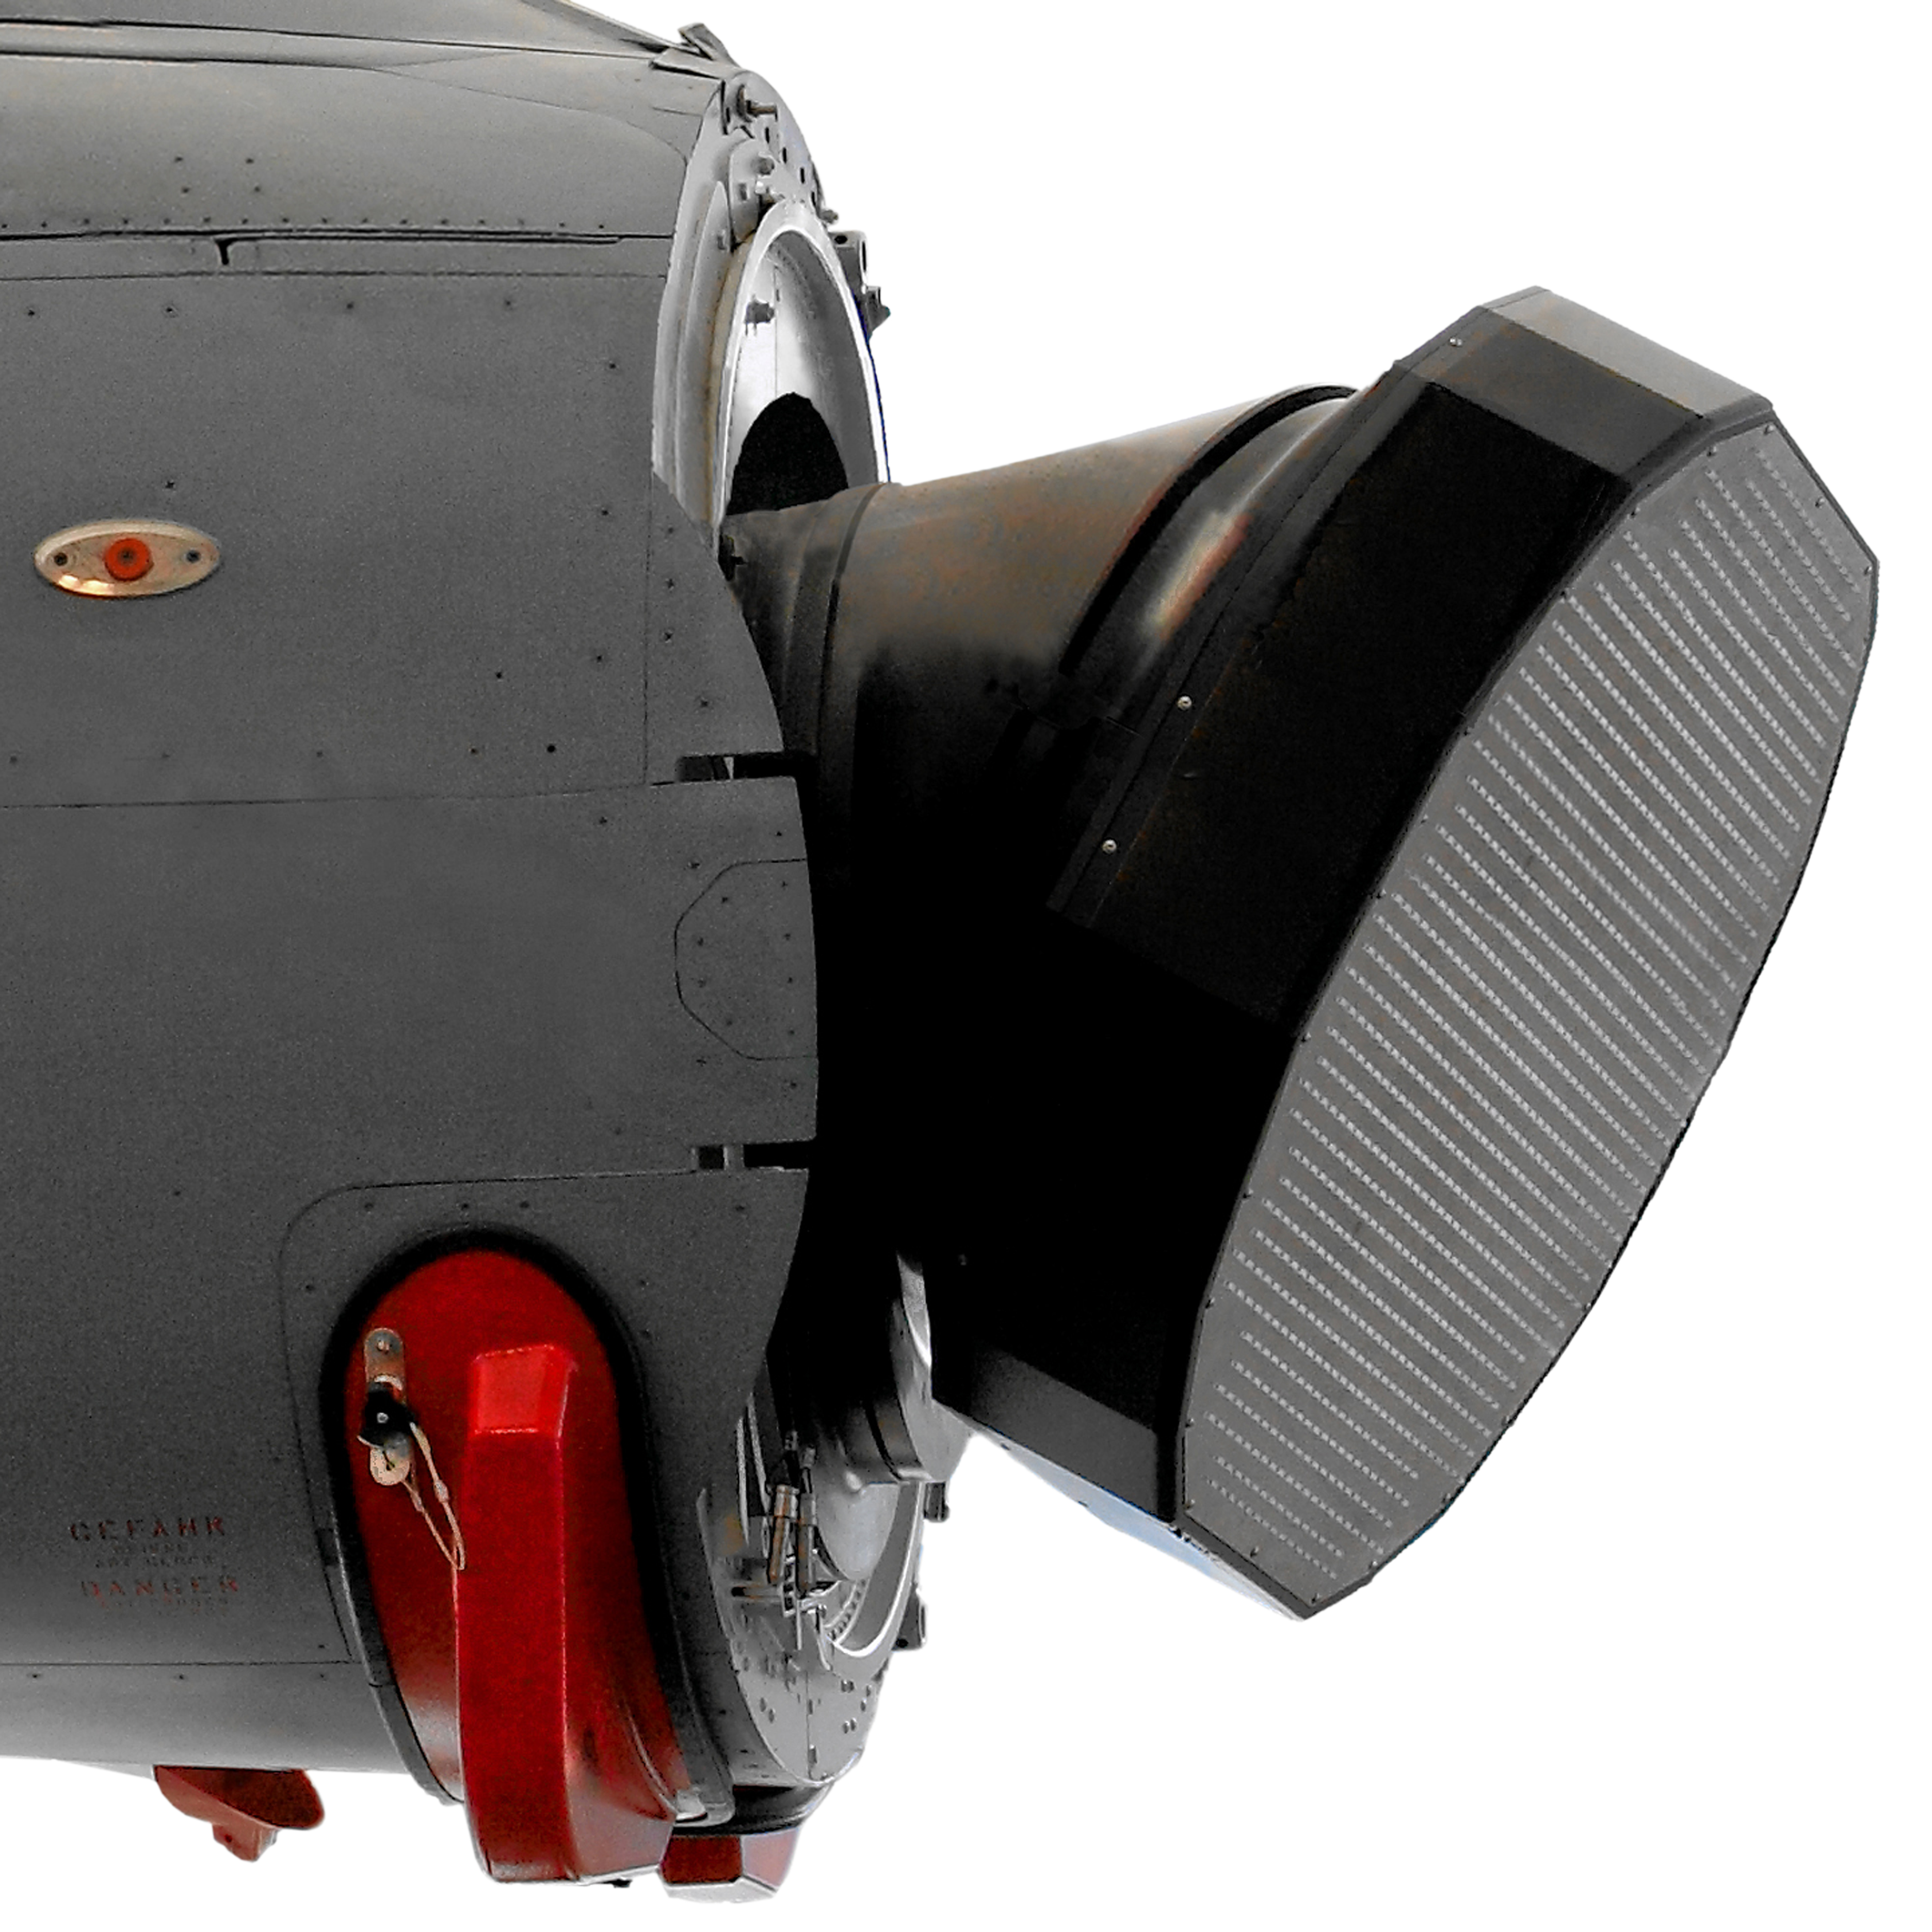
\includegraphics[max width=\linewidth]{gfx/pictures/ILA_Berlin_2012_PD_193-Detail-2}
        \caption{AESA antenna CAPTOR-E inside a Eurofighter's nose cone (removed). Source: \url{https://wikimedia.org/wiki/File:ILA_Berlin_2012_PD_193-Detail-2.jpg}}
        \label{fig:aesa}
    \end{subfigure}
    \hfill
    \begin{subfigure}[t]{0.3\textwidth}
        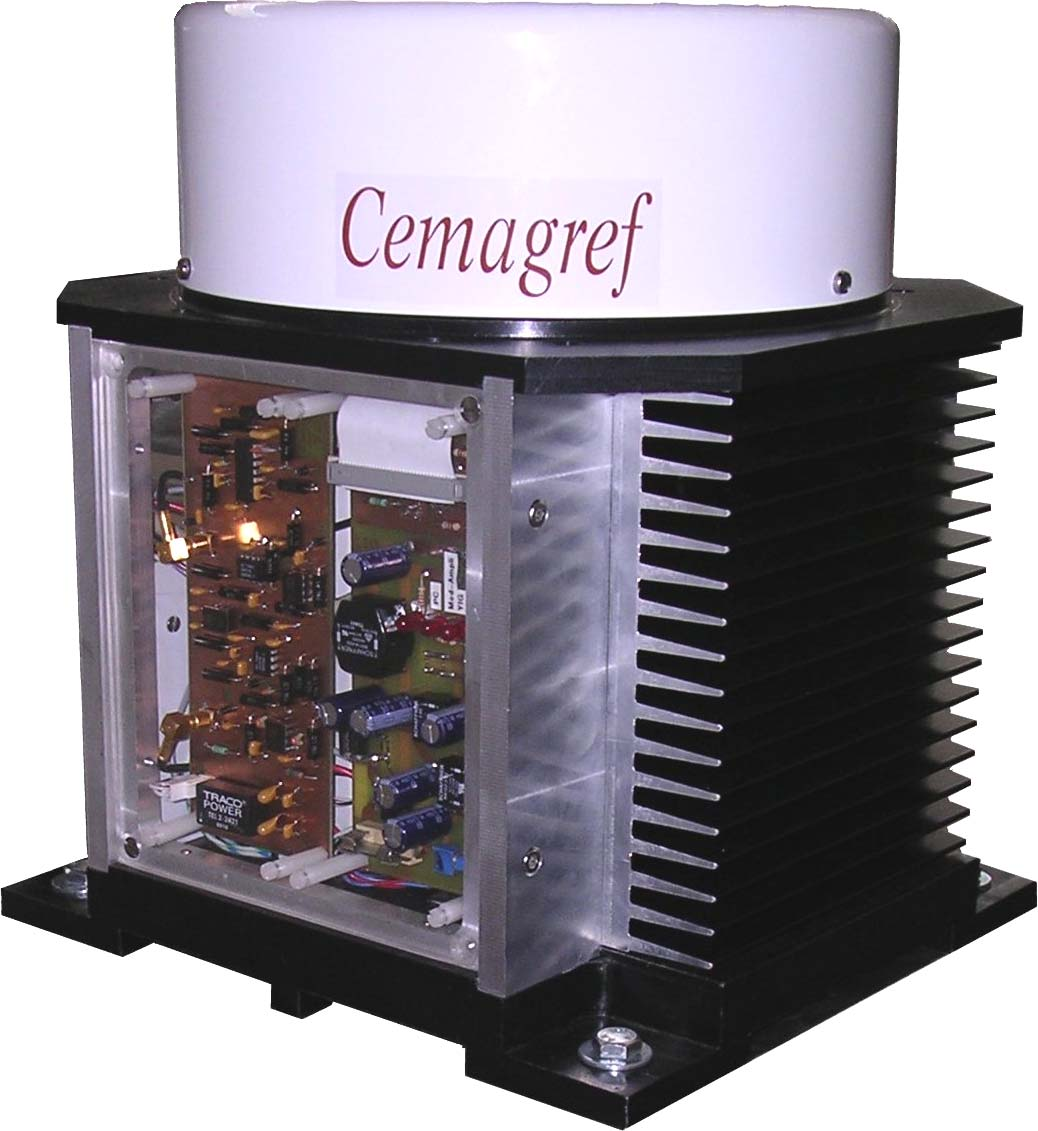
\includegraphics[max width=\linewidth]{gfx/pictures/k2pi}
        \caption{K2PI FMCW radar. Named for operating in the K band frequency (\SI{24}{GHz}) and rotating by $2\pi$ radian. Source: \cite{Rouveure2008}}
        \label{fig:k2pi}
    \end{subfigure}
    \caption{Scanning radars.}
\end{figure}


\subsection{Radar slam}\label{radar-slam}


Simultaneous localization and mapping algorithms are of course a very useful tool in the effort to create an accurate map of a robot's surroundings and have been referred to as the ``holy grail'' of autonomous robotics research \cite{Dissanayake2001}.

Most newer slam navigation algorithms are derived from the classical Bayesian probabilistic recursion. They model the system by a probabilistic density function (PDF) on map and agent location. At the discrete time step $t$ the joint PDF for location $X_t$ and map $M_t$ is based on the history of (noisy) control inputs $U$, state $X$ (usually map location in terms of translation and rotation from known location $X_0$), and exteroceptive measurements of the environment $Z$ \cite{Adams2012}:
\begin{equation} \label{eq:slam}
    P_{t|t}(X_t,M_t|Z_{1:t},U_{1:t-1},X_0)
\end{equation}
Recursive probabilistic solutions then first \textit{predict} the joint state \( P_{t|t-1}(X_t,M_t|Z_{1:t-1},U_{1:t-1},X_0) \) from control inputs and then \textit{correct} the state with the observations, to get the posterior of \cref{eq:slam}.

Many current applications using slam acquire observation data with laser scanners or vision sensors (VSLAM), but this is not an inherent limitation of slam. In fact, any kind of sensor can be used as long as it delivers reproducible data where features can easily be re-detected from different locations.

For feature-based slam algorithms, representative landmarks are extracted from observation data. For multistatic radar sensors \cite{Deissler2013,Deissler2012,Seitz2008,Deissler2009} offer a solution that classifies walls, edges and corners from multipath signal propagation round trip times.

In \cite{Adams2012}, Adams, \textit{et al}. explore robotic navigation and mapping with radar. Grid-based radar mapping is shown to have advantages over other slam sensors, because of its wider beam width and foliage penetration capability. \Cref{fig:missed_detections} shows superimposed radar and lidar scans of the scene in \cref{fig:missed_detections_scene}. Radar tends to spatially blur scene information, but penetrates further than optical sensors (laser, vision) as it is less susceptible to occlusions.\\
\Cref{fig:radar_map} shows occupancy gridmaps collected with a laser-based and a radar-based slam. The concrete walls of the moat in the upper left of the scene as well as foliage was captured much better in the radar gridmap.

\begin{figure}[htbp]
    \centering
    \begin{subfigure}[t]{0.45\textwidth}
        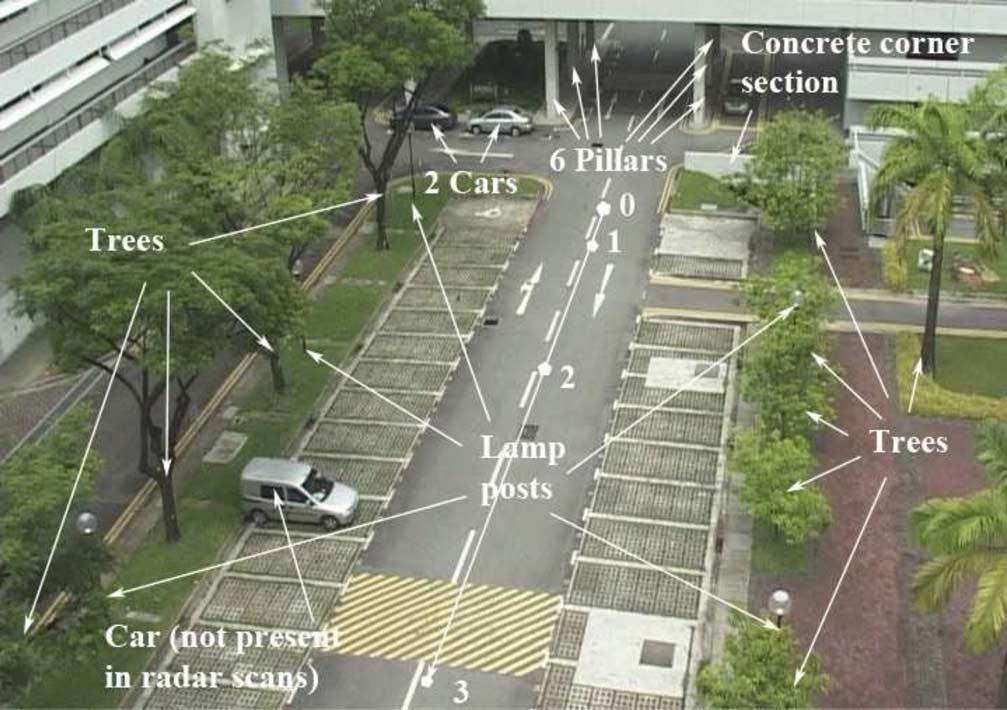
\includegraphics[max width=\linewidth]{pictures/missed_detections_scene}
        \caption{Picture of the scene on the right. Source: \cite{Jose2010}}
        \label{fig:missed_detections_scene}
    \end{subfigure}
    \hfill
    \begin{subfigure}[t]{0.45\textwidth}
        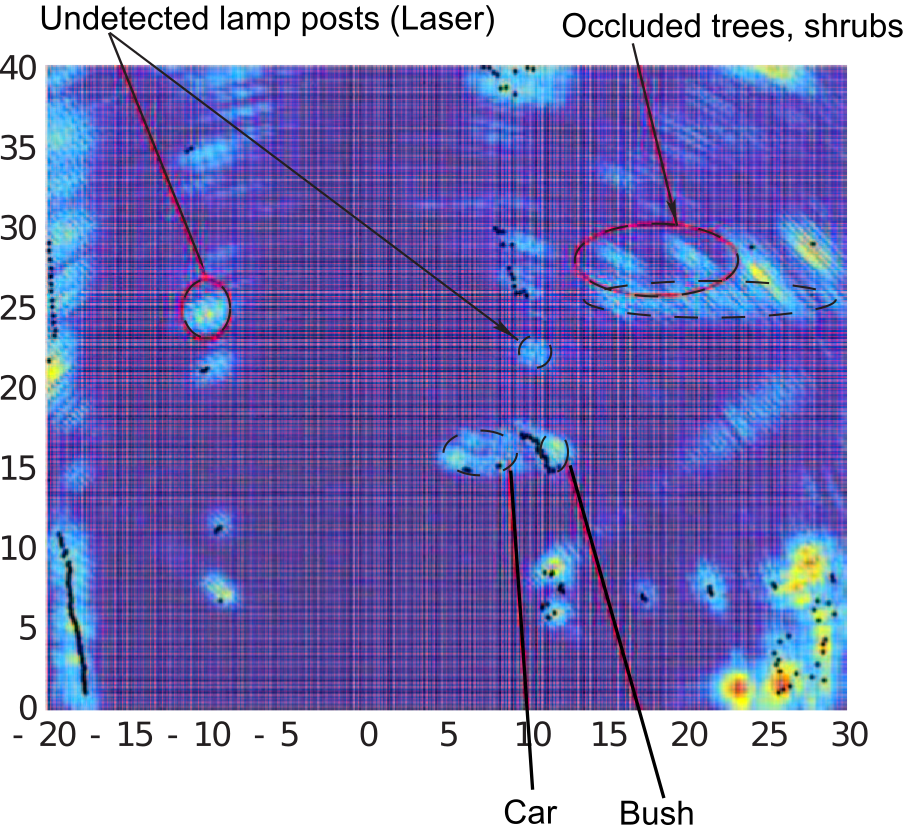
\includegraphics[max width=\linewidth]{diagrams/missed_detections}
        \caption{Radar (heatmap) has fewer missed detections than lidar (black dots), because of its wider beam width and foliage penetration capability. Adapted from \cite{Adams2015}}
        \label{fig:missed_detections}
    \end{subfigure}
    \caption{Superimposed radar and lidar plan position indicator display.}
\end{figure}
\begin{figure}[htbp]
    \centering
    \begin{subfigure}[t]{0.32\textwidth}
        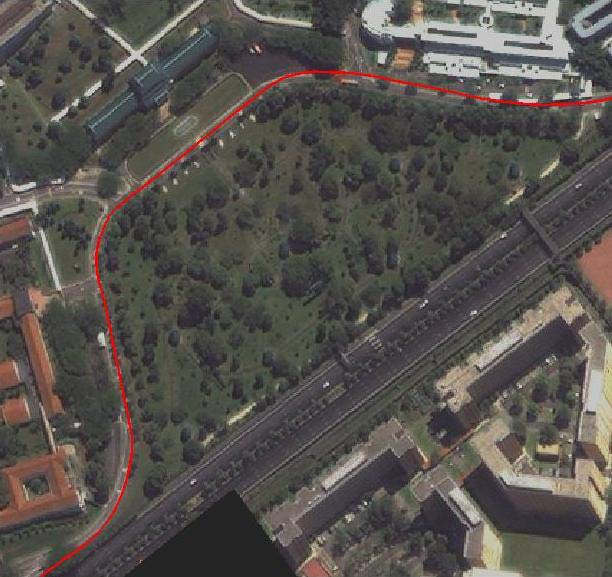
\includegraphics[max width=\linewidth]{diagrams/radar_map_1}
        \caption{Aerial image of the scene}
        \label{fig:radar_map_1}
    \end{subfigure}
    \hfill
    \begin{subfigure}[t]{0.32\textwidth}
        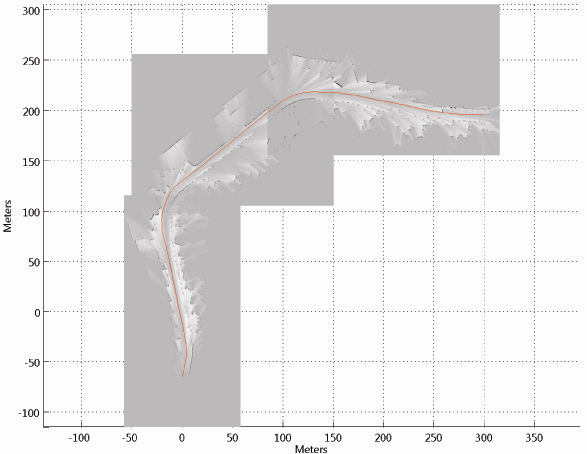
\includegraphics[max width=\linewidth]{diagrams/radar_map_2}
        \caption{Laser based gridmap}
        \label{fig:radar_map_2}
    \end{subfigure}
    \hfill
    \begin{subfigure}[t]{0.32\textwidth}
        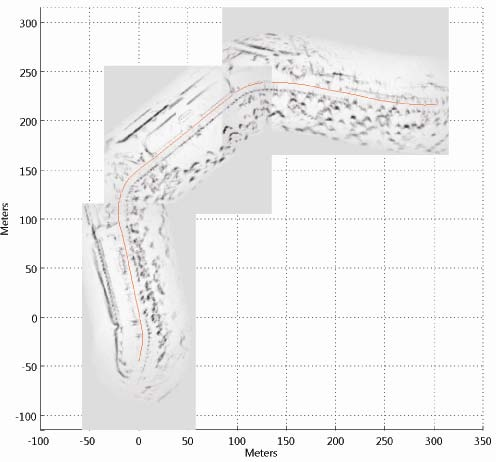
\includegraphics[max width=\linewidth]{diagrams/radar_map_3}
        \caption{Radar based gridmap}
        \label{fig:radar_map_3}
    \end{subfigure}
    \caption{Comparison of radar and lidar occupancy gridmaps. Source: \cite{Adams2015}}
    \label{fig:radar_map}
\end{figure}
